\subsection{Spielinhalt}\label{sec:game-content}
In diesem Kapitel wird der Inhalt des Spiels näher beschrieben. Das Spiel lässt sich primär in zwei Kernmechaniken unterteilen. Das virtuelle Haustiersystem und das Kampfsystem. Diese lassen sich wiederum in Unterkategorien unterteilen, welche in dieser Arbeit untersucht werden.\\

Digimon World bedient sich der Standard-Funktionen für virtuelle Haustiere. Das bedeutet, dass der virtuelle Partner Hunger bekommt, auf die Toilette und schlafen muss. Ebenfalls kann der virtuelle Partner bei mangelnder Pflege erkranken und muss danach mit Medizin versorgt werden.
Diese Bedürfnisse werden in Digimon World vom Partner in Form einer Sprechblase ausgedrückt. Hier liegt bereits der erste Unterschied in den Handbüchern. Während das japanische Handbuch auf Seite 17 fünf verschiedene Bedürfnisse auflistet - Haufen, Essen, Schlaf, Verletzung und Krankheit - listen die anderen beiden Handbücher noch ein sechstes Bedürfnis auf. Diese sind in der amerikanischen Fassung ebenfalls auf Seite 17 zu finden und in der deutschen Fassung auf Seite 19. Das Bedürfnis Müdigkeit besitzt eine andere Hintergrundfarbe und Qualität. Es wurde vermutlich aufgrund von Missverständnissen im Handbuch aufgenommen.\\

\begin{figure}[H]
\begin{center}
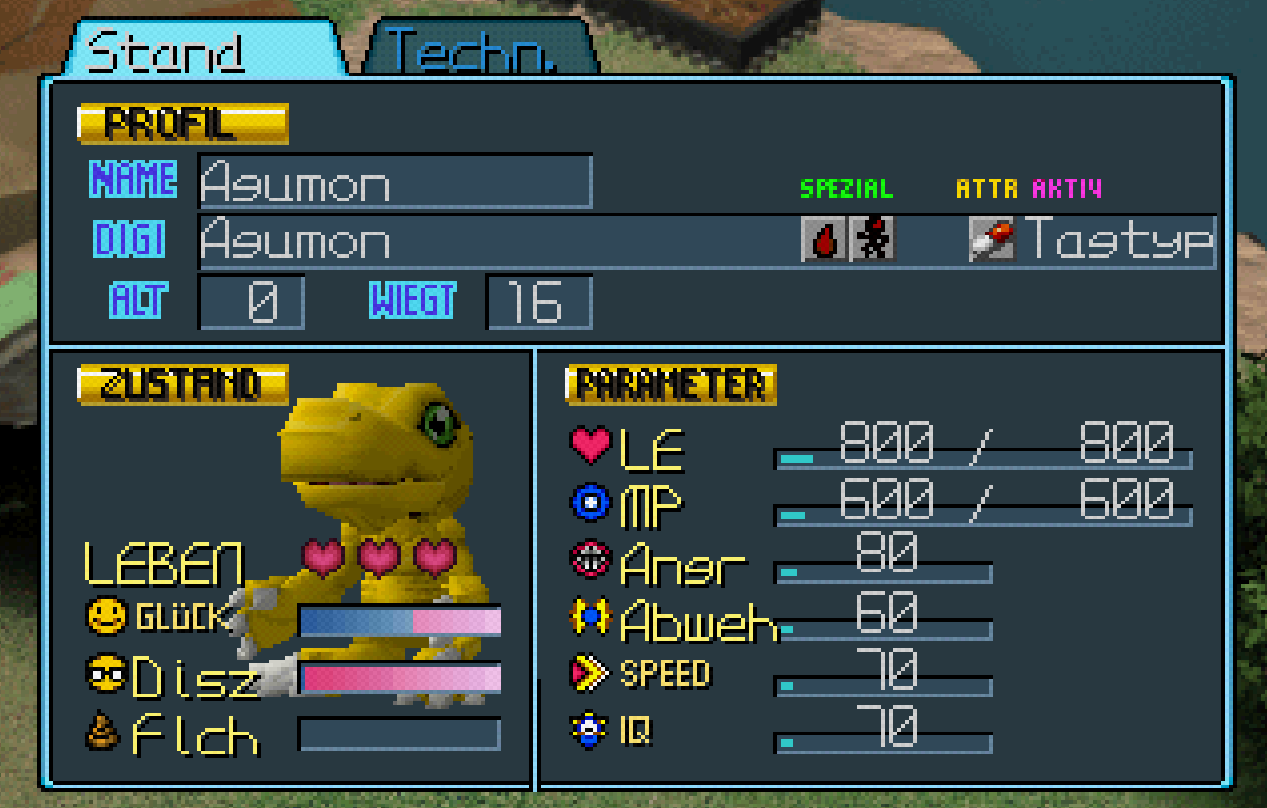
\includegraphics[width=0.8\columnwidth]{figures/screenshots/parameter.png}
  \caption{\label{fig:dw1-parameter} Digimon World: Statusmenü}
\end{center}
\end{figure}

Das Partner-Digimon besitzt weitere Parameter, welche den aktuellen Status näher beschreiben. Diese sind in \autoref{fig:dw1-parameter} in Zustand und Parameter unterteilt. Das aktuelle Glück des Partners verändert seine Lebenserwartung. Ist der Wert höher, lebt das Digimon länger. Der Wert selbst kann durch Loben erhöht werden. Allerdings sinkt dadurch die Disziplin. Eine niedrige Disziplin kann dafür sorgen, dass ein Digimon Gegenstände verweigert. Dazu zählen verschiedene Gegenstände, wie zum Beispiel Nahrungsmittel oder Gegenstände mit dauerhafter Wirkung. Ein hoher Wert führt dazu, dass es eine kürzere Lebenserwartung hat. Mithilfe der Tadeln-Funktion ist es möglich, diesen Wert zu erhöhen. Allerdings verringert sich der Wert des Glücks, außer in zwei Ausnahmen. Wenn das Digimon einen Gegenstand verweigert oder nicht in einer Toilette defäkiert. In der US-Version des Spiels erhöht sich beim korrekten Tadeln das Glück zusätzlich. \\

Ein weiterer Teil von Digimon World sind Elemente aus Rollenspielen. Dazu zählt die Entwicklung des Partner-Digimons, das Abschließen von Aufgaben (Quests) und echtzeitbasierte Kampfmechaniken. Die Hauptquest des Spiels ist es, der Stadt einen bestimmten Wohlstand zu bringen und den letzten Gegner im Spiel zu besiegen. Der Wohlstand wird erhöht, wenn ein Digimon in die Stadt eingeladen wird. Die Stadt erweitert sich schrittweise um bestimmte Funktionalitäten. Beispielhafte Funktionen sind ein Gegenstandsladen, der Transport in andere Gebiete oder eine Klinik.\\

\begin{figure}[H]
\begin{center}
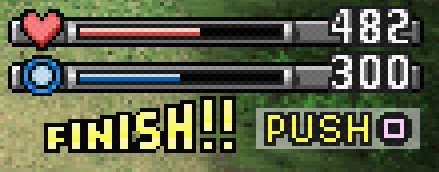
\includegraphics[width=0.7\columnwidth]{figures/screenshots/battle-parameter.png}
  \caption{\label{fig:dw1-battle-parameter} Digimon World: Lebens-, Magie- und Finisheranzeige}
\end{center}
\end{figure}

Das Digimon besitzt Parameter, welche das Kampfgeschehen beeinflussen. Die Lebens- und Magieanzeige gibt an, wie viel Leben oder Magie das Digimon aktuell im Kampf besitzt. Diese sind in \autoref{fig:dw1-battle-parameter} zu sehen. Der Angriffs- und Verteidigungswert beeinflussen die Schadensberechnung. Der Code für diese Berechnung wurde auf Anfrage reverse engineered und hochgeladen\cite{calculatedamage}. Die Formel für die Berechnung eines normalen Angriffs lautet

\begin{equation}
 \frac{T \cdot \frac{P + \frac{D \cdot P}{500}}{30} \cdot (RNG + 90)}{100}   
\end{equation}

und kann durch Ausklammern und Umstellen vereinfacht werden:

\begin{equation}
  \frac{\frac{T}{30} \cdot  P \cdot (1 + \frac{D}{500}) \cdot (RNG + 90)}{100}
\end{equation}

Der Typ-Faktor $T$ bezeichnet den Wert, welcher aus der Summe von drei Spezialisierungen des Verteidigers gebildet wird. Ein Typ beschreibt die im Spiel vorhandenen Elemente, wie zum Beispiel Feuer oder Luft. Alle weiteren Spezialisierungen sind im Handbuch aufgelistet. Der Anfgriffswert $P$ repräsentiert die rohe Kraft einer bestimmten Attacke. $D$ wird berechnet durch die Differenz zwischen dem Angriffswert des Angreifers und dem Verteidigungswert des Verteidigers, wobei $D$ zwischen $-500$ und $500$ liegt. Der Zufallsfaktor $RNG$ wird mithilfe der Funktion \texttt{random(21)} berechnet und befindet sich im Intervall $[0, 20]$.\\

Die Finisheranzeige in \autoref{fig:dw1-battle-parameter} lädt sich Schritt für Schritt anhand unterschiedlicher Wege im Kampf auf. Dabei erscheinen schrittweise die Buchstaben, um das Wort \texttt{FINISH} auszuschreiben. Der erste Weg ist, eine bestimmte Anzahl von Zeit im Kampf zu verbringen. Ein weiterer Weg ist, einen Angriff erfolgreich auszuführen. Zuletzt ist es möglich diese aufzuladen, wenn ein Angriff erfolgreich verteidigt wird. Wenn die Finisheranzeige aufgeladen ist, kann die spielende Person diese mit der angezeigten Taste verbrauchen und einen besonderen Angriff auslösen. Die Ausführung benötigt eine kurze Aufladezeit. Wenn dieser Angriff beim Start unterbrochen wird, verfällt der besondere Angriff. Ansonsten bleibt das gegnerische Digimon stehen und wartet, bis das Partner-Digimon den Angriff ausgeführt hat. Während der Aufladezeit kann die spielende Person abwechselnd die Schultertasten \texttt{L1} und \texttt{R1} betätigen.
Die maximale Aufladung sind zehn Balken. Für die maximale Aufladung benötigt die spielende Person 40 Tastenanschläge in $\approx 6$ Sekunden. Diese Aufladung wird dann mit der rohen Angriffskraft und weiteren Faktoren multipliziert.\\

Eine Kampfsituation tritt ein, wenn der spielbare Charakter ein feindliches Digimon berührt. Danach wird, anhand des aktuell sichtbaren Kamerasichtfelds, die Kampfzone initialisiert\cite{combat-asm}. Jedes weitere feindliche Digimon, welches sich in einem gewissen Radius befindet, hat eine Chance dem Kampf beizutreten. Der spielbare Charakter tritt zur Seite und der Kampf beginnt. Der Kampf findet zwischen dem Partner-Digimon und $n$ feindlichen Digimon statt. Zu Beginn des Spiels ist es nur möglich, die Optionen \texttt{Digimon vertrauen} oder \texttt{Flucht} auszuwählen. Dabei ist es nicht möglich keine Option zu wählen. Standardmäßig wird \texttt{Digimon vertrauen} am Anfang des Kampfes ausgewählt. Digimon vertrauen bewirkt, dass das Digimon eigenständig handelt und sich wahlweise für unterschiedliche Angriffstechniken oder defensive Strategien entscheidet. Flüchten bewirkt die Flucht aus dem Kampf und senkt Disziplin. Es ist allerdings nicht möglich aus Kämpfen gegen Digimon, welche in die Stadt ziehen können, zu fliehen.\\

An dieser Stelle wird eine Kampfsituation, welche im Spiel vorkommen kann, näher erläutert. Die Ausgangssituation ist, dass die spielende Person mit einem Agumon gegen Kunemon kämpft. Agumon besitzt aufgrund vorheriger Kämpfe 649 von 800 Lebenspunkten und 450 von 600 Magiepunkten. Das gegnerische Kunemon startet mit vollen Lebenspunkten. Konkret sind dies 900 Lebenspunkte. Der Kampf startet und die spielende Person wählt die Option \texttt{Digimon vertrauen} aus. Danach läuft Agumon auf Kunemon zu und greift diesen mit der Technik \texttt{Feuerspeier} an, welche eine rohe Angriffskraft von 66 Punkten besitzt. Ebenfalls kostet der Einsatz dieser Fähigkeit 30 Magiepunkte, weswegen Agumon nur noch 420 Magiepunkte besitzt. Kunemon wehrt diesen Angriff allerdings ab, weswegen kein Schaden kalkuliert wird. Agumon verwendet ein weiteres Mal \texttt{Feuerspeier} und fügt Kunemon 71 Schaden zu. Der Rückstoß des Angriffs sorgt dafür, dass Kunemon zurückgestoßen wird. Kunemon bewegt sich auf Agumon zu und versucht einen Nahkampfangriff auszuführen. Allerdings unterbricht ein weiterer \texttt{Feuerspeier} diesen und Kunemon erleidet erneut 70 Schaden. Das bedeutet, dass Kunemon nur noch 759 Lebenspunkte besitzt.\\

Nach einigen weiteren Angriffen besitzt Kunemon 262 und Agumon 286 Lebenspunkte. Aus diesem Grund entscheidet sich die spielende Person, eine kleine Heildisk im Kampf zu verwenden, welche 500 Lebenspunkte heilt. Agumon besitzt dank dieser Heildisk wieder 786 von 800 Lebenspunkten. Während des Kampfes hat sich ebenfalls die Finisheranzeige aufgeladen. Die spielende Person entscheidet sich, diese aufzubrauchen und Agumon startet die Technik \texttt{Pfeffer + Salz}, welche 89 rohen Angriffsschaden verursacht. Die spielende Person betätigt die Schultertasten abwechselnd so schnell wie möglich, aber schafft es nur neun der zehn Balken aufzufüllen. Agumon verwendet die Technik und fügt Kunemon 366 Schaden zu. Kunemon sinkt dadurch auf null Lebenspunkte und der Kampf endet. \\

Die Anzahl an Optionen den Kampf zu manipulieren steigt mit einem höheren Intelligenzwert. Bei einer Intelligenz von 100 ist es möglich, dem Partner zu befehligen, immer den stärksten Angriff zu verwenden. Ein Wert von 200 bewirkt das Gegenteil und der Partner verwendet immer den schwächsten Angriff. Dies kann nützlich sein, wenn man die Magiepunkte langsamer aufbrauchen möchte. Die Möglichkeiten defensiver zu spielen, werden bei einem Wert von 300 und 400 freigespielt. Ab diesem Zeitpunkt ist möglich, dem Partner zu befehligen, auzuweichen oder zu verteidigen. Ebenfalls wird die Option freigeschaltet, manuell den Fokus zwischen mehreren Gegner zu wechseln. Ab einem Intelligenzwert von 500 werden die beiden Optionen, welche bei 100 und 200 freigeschaltet wurden, durch die verfügbaren Kampffertigkeiten ersetzt. Der letzte Wert von 999 erweitert das Repertoire an Optionen nicht, allerdings senkt dieser die Kosten für die Verwendung von Kampffertigkeiten. Das Erlernen von neuen Kampffertigkeiten erfolgt entweder anhand eines höher erreichten Intelligenzwertes oder zufällig im Kampf. Die Wahrscheinlichkeiten, eine Fertigkeit zu Erlernen, sind mithilfe eines Tools einsehbar\cite{move-tool}. \\

\begin{figure}[H]
\begin{center}
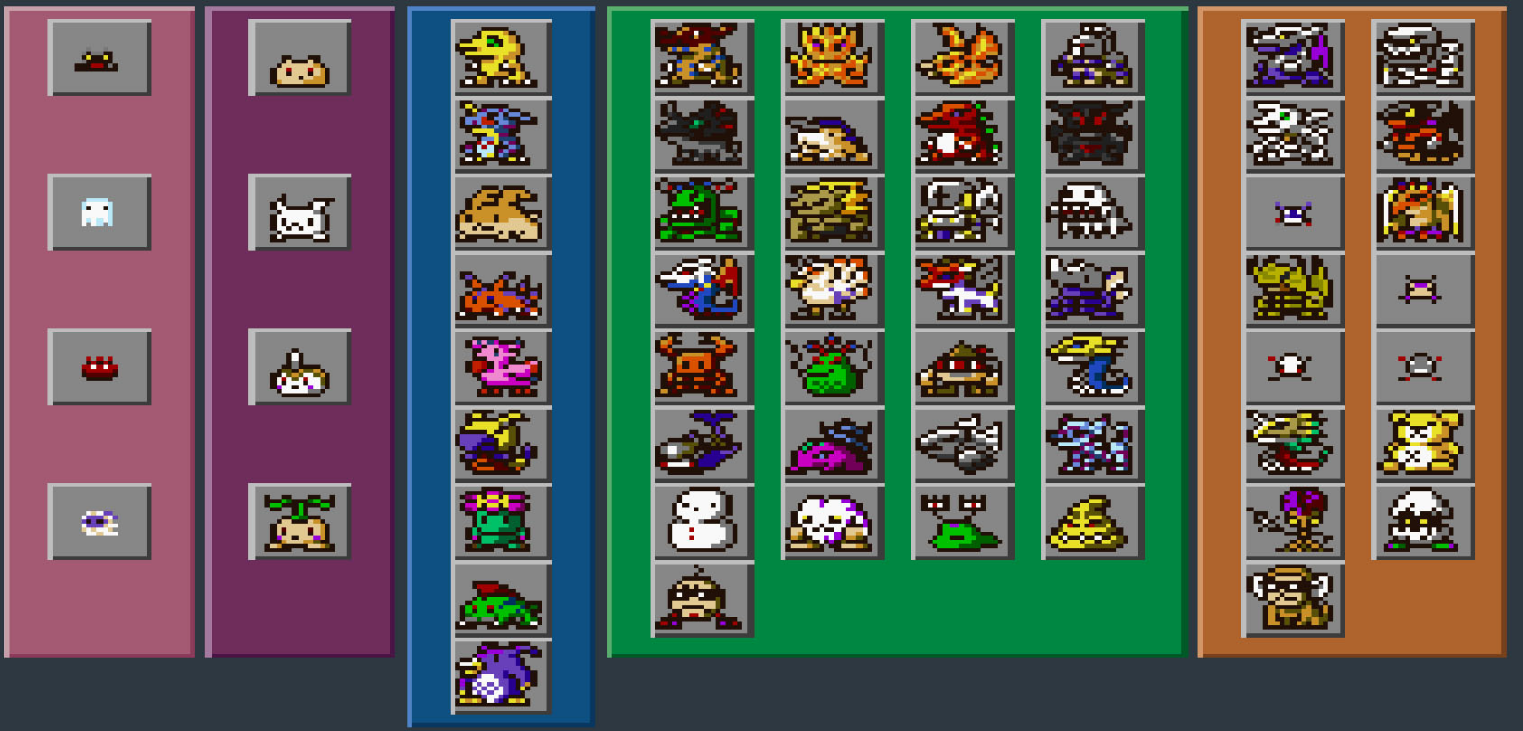
\includegraphics[width=1\columnwidth]{figures/screenshots/digivolutions.png}
  \caption{\label{fig:dw1-digivolutions} Digimon World: Alle Entwicklungsformen}
\end{center}
\end{figure}

Digimon World beinhaltet eine bestimmte Form der Entwicklung. Diese nennt sich Digitation und ist Hauptbestandteil des Digimon-Universums. Diese wird auch im Handbuch des Spiels beschrieben. Digimon durchlaufen verschiedene Entwicklungsstufen, welche in \autoref{fig:dw1-digivolutions} zu sehen sind. Das Handbuch beschreibt die Entwicklung vom Ausbildungs- bis zum Ultralevel. Allerdings wird das Babylevel außer Acht gelassen, welches sich noch vor dem Ausbildungslevel stattfindet. Die Digitation findet nach einer bestimmten Zeitspanne statt und richtet sich dann nach bestimmten Kriterien. Die Kriterien basieren auf Parametern, wie zum Beispiel Angriffswerten oder Intelligenz, dem aktuellen Gewicht, Pflegefehler und unter Umständen einem Bonuskriterium. Mithilfe eines Tools lassen sich diese Kriterien besser nachverfolgen\cite{digivolution}. \\

Es existieren verschiedene Gegenstände, welche Werte des Partners verändern können. Disks können im und außerhalb des Kampfes verwendet werden und helfen, Kampfparameter wie Lebens- oder Magiepunkte aufzufüllen. Chips sind Gegenstände, welche die maximale Obergrenze von Parametern erhöhen können. Diese Wirkung ist permanent. Nahrungsmittel füllen die Hungerleiste des Digimons wieder auf und besondere Gegenstände wie das Camping-WC sorgen dafür, dass die Toilette überall verwendet werden kann. Zuletzt gibt es noch Gegenstände, welche eine Digitation erzwingen können. Einzelne Gegenstände werden auch in den Handbüchern beschrieben, allerdings fehlen viele Abbildungen in der deutschen Ausgabe.\\

Neben den zahlreichen Gegenständen ist es auch möglich, die Werte durch Digitation, Kämpfe oder Training zu erhöhen. Die gerade beschriebenen Gegenstände, welche eine Digitation erzwingen, erhöhen die Werte allerdings nicht. Das bedeutet, dass es effizienter ist, das Parnter-Digimon ohne Gegenstände zu einem höheren Digitationslevel zu entwickeln. Das Spiel bietet zusätzlich viele verschiedene Trainingsareale, welche helfen, die Werte des Partner-Digimons zu erhöhen. Konkrete Informationen zum Training können mithilfe eines Tools berechnet werden\cite{dw-training}. Durch Kämpfe ist es ebenfalls möglich, an höhere Werte zu kommen. Allerdings sind diese im Vergleich zum Training wenig effizient.\\

Im Spiel existieren noch weitere Funktionen, wie das Sammeln von Karten, Medaillen oder das Bestreiten von Turnieren. In den Turnieren kann der Kampf mithilfe der Memory Card\footnote{Speicherkarte für die \ac{PSX}} gegen eine weitere Person ausgetragen werden. Allerdings werden diese Funktionen in der Bachelorarbeit bewusst nicht berücksichtigt. Das liegt daran, dass diese Funktionalitäten nicht relevant für den Prototypen und das fertige Produkt sind.\\